\section{Methodology and Evaluation}
\label{sec:methodology}
\emph{\color{red}Methodology and evaluation: how do you plan to evaluate whether your hypothesis is correct?}

\begin{figure}[t]
      \centering
      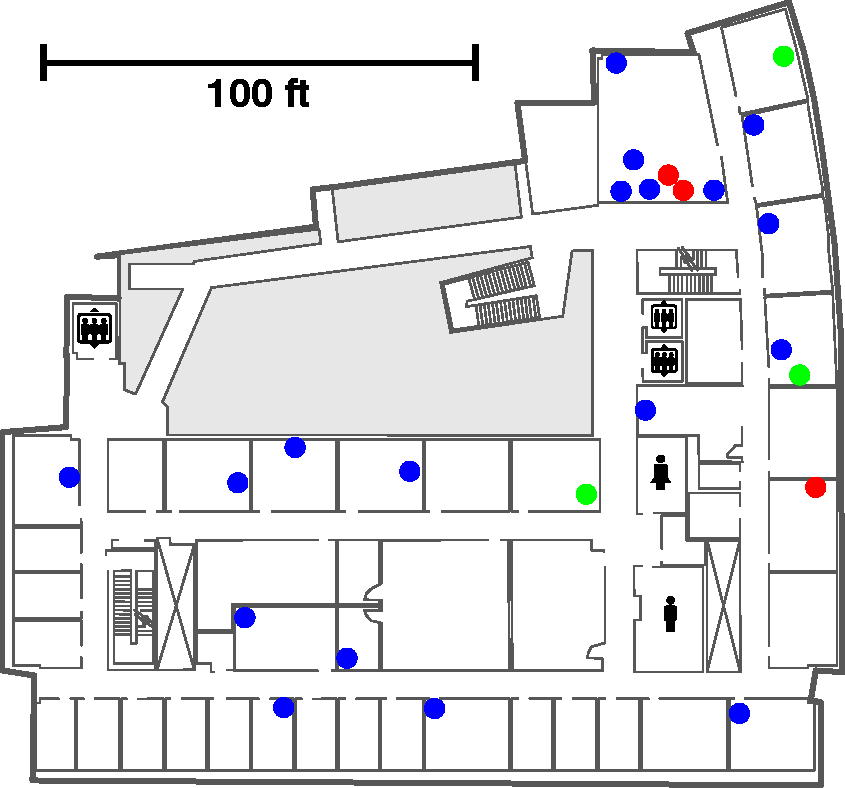
\includegraphics[width=0.8\columnwidth]{figures/floor3_grayscale_noee_testbed.pdf}
      \caption{\label{fig:testbed} Our indoor 802.11n testbed at UW CSE consists of 22 nodes spread over 3 color-coded floors. The nodes are placed to ensure a large number of links between them, a variety of distances between nodes, and diverse scattering characteristics.}
\end{figure}


\heading{802.11n Wireless Testbed.}

\heading{Compare to Spatial Reuse.}
CMAP~\cite{vutukuru_cmap} and Multiuser MIMO~\cite{heath_mumimo,spencer_mumimo} are two flavors of systems that aim to promote spatial reuse. In most results, these mechanisms offer at best a 2$\times$ improvement in network capacity, at the cost of very complex synchronization mechanisms. In addition, practical work in these areas tends to ignore rate selection and thus may overstate its benefits~\cite{brodsky_csma}. How do we do with multiple channels, or short-circuiting topologies, and how much better can we do with these additional mechanisms?